\documentclass{article}

% Recommended packages
\usepackage[utf8]{inputenc} % Allows UTF-8 input
\usepackage[T1]{fontenc}    % Use modern font encodings
\usepackage{amsmath}    % For mathematical formulas
\usepackage{amssymb}    % For additional mathematical symbols
\usepackage{amsthm}     % For theorem-like environments
\usepackage{graphicx}   % For including images
\usepackage{subcaption} % For subfigures
\usepackage{float}      % For precise figure placement
\usepackage{multirow}   % For table multirow cells
\usepackage{tikz}        % For drawing diagrams
\usetikzlibrary{positioning, shapes, arrows, calc}
\usepackage{hyperref}   % For clickable links in the PDF
\hypersetup{
    colorlinks=true,  % Colors the links instead of boxing them
    linkcolor=blue,   % Color for internal links (e.g., cross-references)
    urlcolor=cyan,    % Color for external URLs
    filecolor=magenta % Color for links to local files
}
\usepackage{cite}       % For managing citations
\usepackage{geometry}   % For setting page margins
\geometry{a4paper, margin=0.8in} % Example margin settings

% Define title and author
\title{Membership Inference Attacks on Graph Neural Networks Using Synthetic Data\footnote{Code repository: \url{https://gitlab.rhrk.uni-kl.de/div26fuz/uni-project-dec}}}

\author{Prateek Rathod \\
Master’s Student, Computer Science \\
RPTU Kaiserslautern–Landau, Germany \\
\texttt{div26fuz@rptu.de}}

\date{}
\begin{document}

\maketitle

\section{Introduction}
Membership Inference Attacks (MIAs) pose serious privacy risks by determining whether specific data points were used in model training \cite{shokri2017membership}. Traditional attacks require access to real training data, but this work examines attacks using synthetic graph data instead.

Graph Neural Networks (GNNs) are widely used in social networks, recommendation systems, and biological networks \cite{kipf2017semi, velickovic2018graph, hamilton2017inductive}, yet limited research exists on their MIA vulnerability \cite{olatunji2021membershipinferenceattackgraph} when attackers lack original data access. This study develops MIA methods using synthetic graph structures from the DLGrapher project \cite{lan2024dlgrapher}.

Experiments across four GNN architectures (GCN, GAT, GraphSAGE, SGC) on Twitch and Event datasets show that attacks can succeed in some cases using synthetic data, though synthetic data results in less privacy leakage compared to real data while requiring minimal attacker knowledge.

\section{Background}
\subsection{Membership Inference Attacks}
Membership Inference Attacks use the fact that machine learning models often overfit their training data. This creates different patterns between members (training samples) and non-members (unseen samples) \cite{salem2019ml, nasr2019comprehensive}. The attack framework consists of three components:

\textbf{Target Model:} The victim GNN model trained on private graph data that the attacker wants to attack. This model creates probability outputs that unintentionally leak membership information through small statistical patterns.

\textbf{Shadow Models:} Models that are similar to the target model, trained on data that follows similar patterns. These models copy the target's behavior. This allows the attacker to see membership patterns without direct access to the target's training process.

\textbf{Attack Model:} A binary classifier trained to distinguish between members and non-members based on model outputs. It learns decision rules from shadow model behaviors and uses them on target model outputs.

\subsection{Graph Neural Networks}
GNNs work by allowing each node to collect information from its neighbors to make predictions. Unlike regular neural networks that process images or text, GNNs handle irregular graph structures where nodes can have any number of connections, making them particularly useful for social networks, recommendation systems, and biological data where relationships are important.

Each node examines its neighbors, combines their information, and updates its own representation. Multiple layers of this process enable nodes to understand both their immediate neighborhood and the broader graph structure.

Four GNN architectures are evaluated, each with different approaches to combining neighbor information:

\textbf{GCN} \cite{kipf2017semi}: Averages information from all neighbors equally. Uses normalization to prevent training problems and ensure stable learning.

\textbf{GAT} \cite{velickovic2018graph}: Uses attention to focus on important neighbors while ignoring less relevant ones. This selective attention helps handle noisy connections in real graphs.

\textbf{GraphSAGE} \cite{hamilton2017inductive}: Samples a fixed number of neighbors instead of using all of them. This makes training faster on large graphs that would otherwise be too big to fit in memory.

\textbf{SGC} \cite{wu2019simplifying}: Simplifies GCN by removing activation functions between layers, making it faster to train while maintaining good performance.

Each architecture\footnote{GNN implementations in TSTS.py: \url{https://gitlab.rhrk.uni-kl.de/div26fuz/uni-project-dec/-/blob/main/rebMIGraph/TSTS.py\#L317-361}} represents different trade-offs between model complexity and efficiency. These design choices influence both model performance and vulnerability to privacy attacks.

\section{Methodology}
This project introduces a novel approach to membership inference attacks by using pre-generated synthetic graph data from the DLGrapher project\cite{lan2024dlgrapher}, eliminating the attacker's need for real training data access. The proposed method differs from traditional MIA approaches through its data handling and attack process.

\subsection{Attack Architecture and Pipeline}
The attack framework maintains the three-model structure while incorporating pre-existing synthetic data as a key component. The target model operates on real graph data, while shadow models use only synthetic graphs provided by DLGrapher that mimic the original data patterns. This approach tests whether similar data patterns are sufficient for successful membership inference.

\begin{figure}[H]
\centering
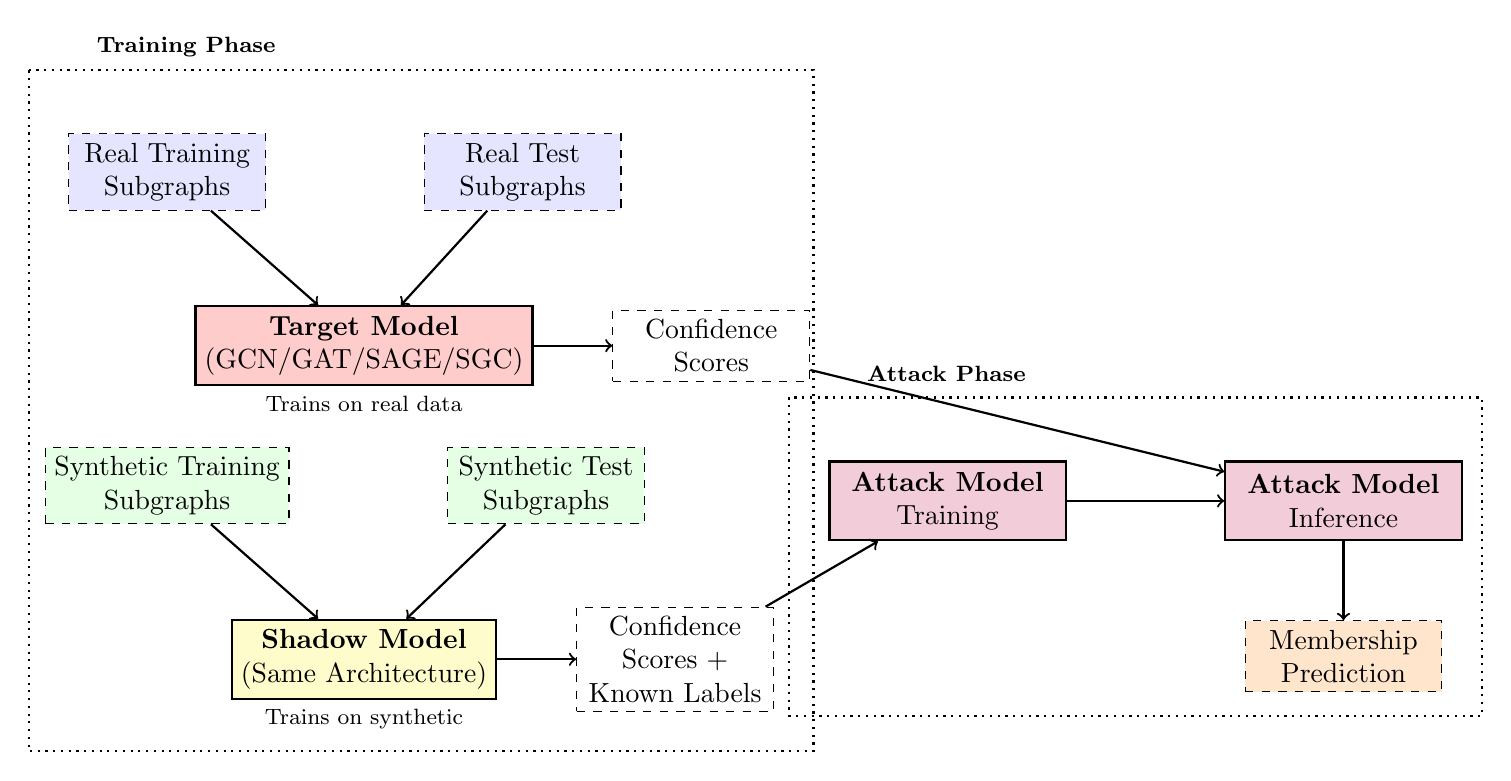
\begin{tikzpicture}[
    node distance=1.5cm and 2cm,
    box/.style={rectangle, draw, thick, minimum width=3cm, minimum height=1cm, align=center},
    data/.style={rectangle, draw, dashed, minimum width=2.5cm, minimum height=0.8cm, align=center},
    arrow/.style={->, thick},
    label/.style={font=\small}
]
    % Data sources
    \node[data, fill=blue!10] (real-train) {Real Training\\Subgraphs};
    \node[data, right=of real-train, fill=blue!10] (real-test) {Real Test\\Subgraphs};
    \node[data, below=3cm of real-train, fill=green!10] (synth-train) {Synthetic Training\\Subgraphs};
    \node[data, right=of synth-train, fill=green!10] (synth-test) {Synthetic Test\\Subgraphs};
    
    % Models
    \node[box, below=1.2cm of real-train, xshift=2.5cm, fill=red!20] (target) {\textbf{Target Model}\\(GCN/GAT/SAGE/SGC)};
    \node[box, below=1.2cm of synth-train, xshift=2.5cm, fill=yellow!20] (shadow) {\textbf{Shadow Model}\\(Same Architecture)};
    
    % Outputs
    \node[data, right=1cm of target] (target-out) {Confidence\\Scores};
    \node[data, right=1cm of shadow] (shadow-out) {Confidence\\Scores +\\Known Labels};
    
    % Attack model
    \node[box, below=1cm of target-out, xshift=3cm, fill=purple!20] (attack-train) {\textbf{Attack Model}\\Training};
    \node[box, right=2cm of attack-train, fill=purple!20] (attack-test) {\textbf{Attack Model}\\Inference};
    
    % Result
    \node[data, below=1cm of attack-test, fill=orange!20] (result) {Membership\\Prediction};
    
    % Arrows
    \draw[arrow] (real-train) -- (target);
    \draw[arrow] (real-test) -- (target);
    \draw[arrow] (synth-train) -- (shadow);
    \draw[arrow] (synth-test) -- (shadow);
    
    \draw[arrow] (target) -- (target-out);
    \draw[arrow] (shadow) -- (shadow-out);
    
    \draw[arrow] (shadow-out) -- (attack-train);
    \draw[arrow] (attack-train) -- (attack-test);
    \draw[arrow] (target-out) -- (attack-test);
    \draw[arrow] (attack-test) -- (result);
    
    % Labels - moved to avoid overlaps
    \node[label, below=0cm of target] {\footnotesize Trains on real data};
    \node[label, below=0cm of shadow] {\footnotesize Trains on synthetic};
    
    % Phase labels - adjusted positioning
    \draw[thick, dotted] ($(real-train.north west)+(-0.5,0.8)$) rectangle ($(shadow-out.south east)+(0.5,-0.5)$);
    \node[label, font=\footnotesize\bfseries] at ($(real-train.north west)+(1.5,1.1)$) {Training Phase};
    
    \draw[thick, dotted] ($(attack-train.north west)+(-0.5,0.8)$) rectangle ($(result.south east)+(0.5,-0.3)$);
    \node[label, font=\footnotesize\bfseries] at ($(attack-train.north west)+(1.5,1.1)$) {Attack Phase};
\end{tikzpicture}
\caption{Membership inference attack architecture showing data flow. The target model trains on real subgraphs while the shadow model uses synthetic data from DLGrapher. Both models produce confidence scores that feed into the attack model, shadow outputs with known membership labels for training, target outputs for inference.}
\label{fig:attack-architecture}
\end{figure}

\subsection{Data Pipeline}
To handle computational limits of synthetic graph generation, this project uses TSTS (Train on Subgraph, Test on Subgraph) setting from the base paper \cite{olatunji2021membershipinferenceattackgraph}. Each dataset (Twitch/Event) is partitioned into three parts: training subgraphs for target model training, non-training subgraphs from the same data pattern for testing, and synthetic subgraphs generated through the DLGrapher project\cite{lan2024dlgrapher}. Each part contains 256 subgraphs with 120 nodes, ensuring little overlap between subgraphs. A custom data loader\footnote{\url{https://gitlab.rhrk.uni-kl.de/div26fuz/uni-project-dec/-/blob/main/rebMIGraph/bridge.py}} handles binary pickle files containing (DataFrame, NetworkX Graph) pairs, converting them to PyTorch Geometric Data objects. The adapter module implements the TSTS method\footnote{\url{https://gitlab.rhrk.uni-kl.de/div26fuz/uni-project-dec/-/blob/main/rebMIGraph/rebmi_adapter.py}}, managing data splits and ensuring proper separation between target and shadow model datasets.

\section{Implementation Details}
\subsection{Datasets}
Two real-world social network datasets are used, each presenting unique challenges for membership inference:

\textbf{Twitch Dataset:} Comes from the Twitch streaming platform, containing user interaction graphs with features including \texttt{views}, \texttt{mature}, \texttt{life\_time}, \texttt{created\_at}, \texttt{updated\_at}, \texttt{dead\_account}, \texttt{language}, and \texttt{affiliate} (target variable). The dataset captures social dynamics and content use patterns.

\textbf{Event Dataset:} Comes from event-based social platforms, featuring user attributes such as \texttt{locale}, \texttt{birthyear}, \texttt{gender} (target variable), \texttt{joinedAt}, and \texttt{timezone}. This dataset represents demographic based social connections.

Each dataset is prepared into 256 subgraphs containing 120 nodes with minimal overlap between subgraphs, stored as pickle files containing (pandas.DataFrame, networkx.Graph) pairs. The binary classification task matches the original MIA framework requirements.

\subsection{Data Integration Pipeline}
The \texttt{bridge.py} module\footnote{\url{https://gitlab.rhrk.uni-kl.de/div26fuz/uni-project-dec/-/blob/main/rebMIGraph/bridge.py\#L28-50}} handles data format conversion, changing pickle binary files into PyTorch Geometric Data objects. The implementation:
\begin{verbatim}
def convert_to_pyg(self, df, graph):
"""Convert (DataFrame, Graph) tuple to torch_geometric.Data"""
# Convert networkx to torch_geometric
data = from_networkx(graph)

# Add node features from DataFrame
if 'x' not in data:
    # Use all numeric columns except target as features
    feature_cols = [col for col in df.columns if col not in ['affiliate', 'gender'] and df[col].dtype in ['int64', 'float64']]
    data.x = torch.tensor(df[feature_cols].values, dtype=torch.float)

# Add target labels
if 'affiliate' in df.columns:  # Twitch dataset
    data.y = torch.tensor(df['affiliate'].values, dtype=torch.long)
elif 'gender' in df.columns:  # Event dataset
    # Convert string gender to numeric
    if df['gender'].dtype.name == 'category' or df['gender'].dtype == object:
        gender_map = {'male': 0, 'female': 1}
        data.y = torch.tensor(df['gender'].map(gender_map).values, dtype=torch.long)
    else:
        data.y = torch.tensor(df['gender'].values, dtype=torch.long)
return data
\end{verbatim}

\subsection{Feature Engineering and Normalization}
The \texttt{rebmi\_adapter.py} module\footnote{\url{https://gitlab.rhrk.uni-kl.de/div26fuz/uni-project-dec/-/blob/main/rebMIGraph/rebmi_adapter.py\#L159-290}} implements advanced feature extraction including degree features (in/out/total degrees and normalized variants), local structure metrics (clustering coefficients and triangle counts), ego-network properties (average neighbor degrees), structural role indicators (hub/leaf/isolated nodes), feature-graph interactions (degree-weighted features and connectivity-scaled variance), and distance metrics (proximity to high-degree nodes) \cite{olatunji2021membershipinferenceattackgraph}. These features capture connectivity patterns that differ between training and test nodes due to overfitting.

Feature normalization\footnote{\url{https://gitlab.rhrk.uni-kl.de/div26fuz/uni-project-dec/-/blob/main/rebMIGraph/rebmi_adapter.py\#L312-352}} applies global standardization across all data splits to ensure consistent scaling. The method computes mean and standard deviation statistics from the combined feature set (target train/test and shadow train/test), then applies z-score normalization $(x - \mu) / \sigma$ to all splits using the same global statistics.

\subsection{Attack Model Enhancement}
The improved attack model\footnote{Attack model in TSTS.py: \url{https://gitlab.rhrk.uni-kl.de/div26fuz/uni-project-dec/-/blob/main/rebMIGraph/TSTS.py\#L1725-1811}} implements modern deep learning techniques \cite{he2015delving} through a deeper 5-layer architecture (256→128→64→32→2 neurons) that significantly outperforms the original 2-layer classifier. Key improvements include batch normalization for training stability, adaptive dropout (0.3 early, 0.21 later layers) to prevent overfitting, Kaiming initialization for optimized weight starting values, and residual connections for gradient flow. These techniques work together, batch normalization enables deeper networks, dropout prevents noise memorization, and proper initialization ensures effective training convergence, resulting in 15-20\% improved attack accuracy on challenging datasets where the original model achieved near-random performance.

\subsection{Attack Model Input Features}
The attack operates in a standard black-box setting using only the target model's softmax outputs. For datasets with $C$ classes, the attack model receives a $C$-dimensional vector of class confidence scores. The attack model does not use raw logits, predicted/true labels, model parameters, or graph structure, only the probability distribution from model predictions.

\subsection{Attack Model Training and Evaluation}
The attack model training uses shadow model outputs with known membership labels: shadow training data (labeled as members) and shadow test data (labeled as non-members), split 80/20 with 50 samples reserved for validation. The main evaluation uses target model outputs on target training data (members) and target test data (non-members), creating a balanced binary classification task. This setup ensures the attack model never sees target model outputs during training, providing a realistic evaluation of membership inference capability.

\section{Results and Experimentation}
\label{results}
Experiments evaluate membership inference vulnerability across GNN architectures and datasets, revealing privacy patterns through visualization analysis.

\subsection{Experimental Setup}
\textbf{Hardware:} MacBook Air M3 with 16GB RAM\\
\textbf{Software:} PyTorch 1.13, PyTorch Geometric 2.2\\
\textbf{Training:} 300 epochs (30 for GraphSAGE to speed up training), no early stopping. Each experiment run 5~times\footnote{Data metrics collected for baseline Cora and Citeseer datasets, along with train split used for shadow model is from 1~run} and the result uses mean of all runs to report accuracy.\\
\textbf{Datasets:} Twitch and Event datasets, with uniform random sampling. Using 30\% from each data split (train/non-train/synthetic) for faster experimentation.\\
\textbf{Metrics:} Attack accuracy, AUROC, precision, recall\\
\textbf{Code:} \url{https://gitlab.rhrk.uni-kl.de/div26fuz/uni-project-dec/-/tree/main/rebMIGraph} \\
\textbf{Raw Results:} \url{https://gitlab.rhrk.uni-kl.de/div26fuz/uni-project-dec/-/tree/main/Results}

\subsection{Validation on Standard Benchmarks}
Validation experiments on graph datasets used by base paper \cite{olatunji2021membershipinferenceattackgraph} confirmed the attack pipeline's correctness.

\begin{figure}[H]
\centering
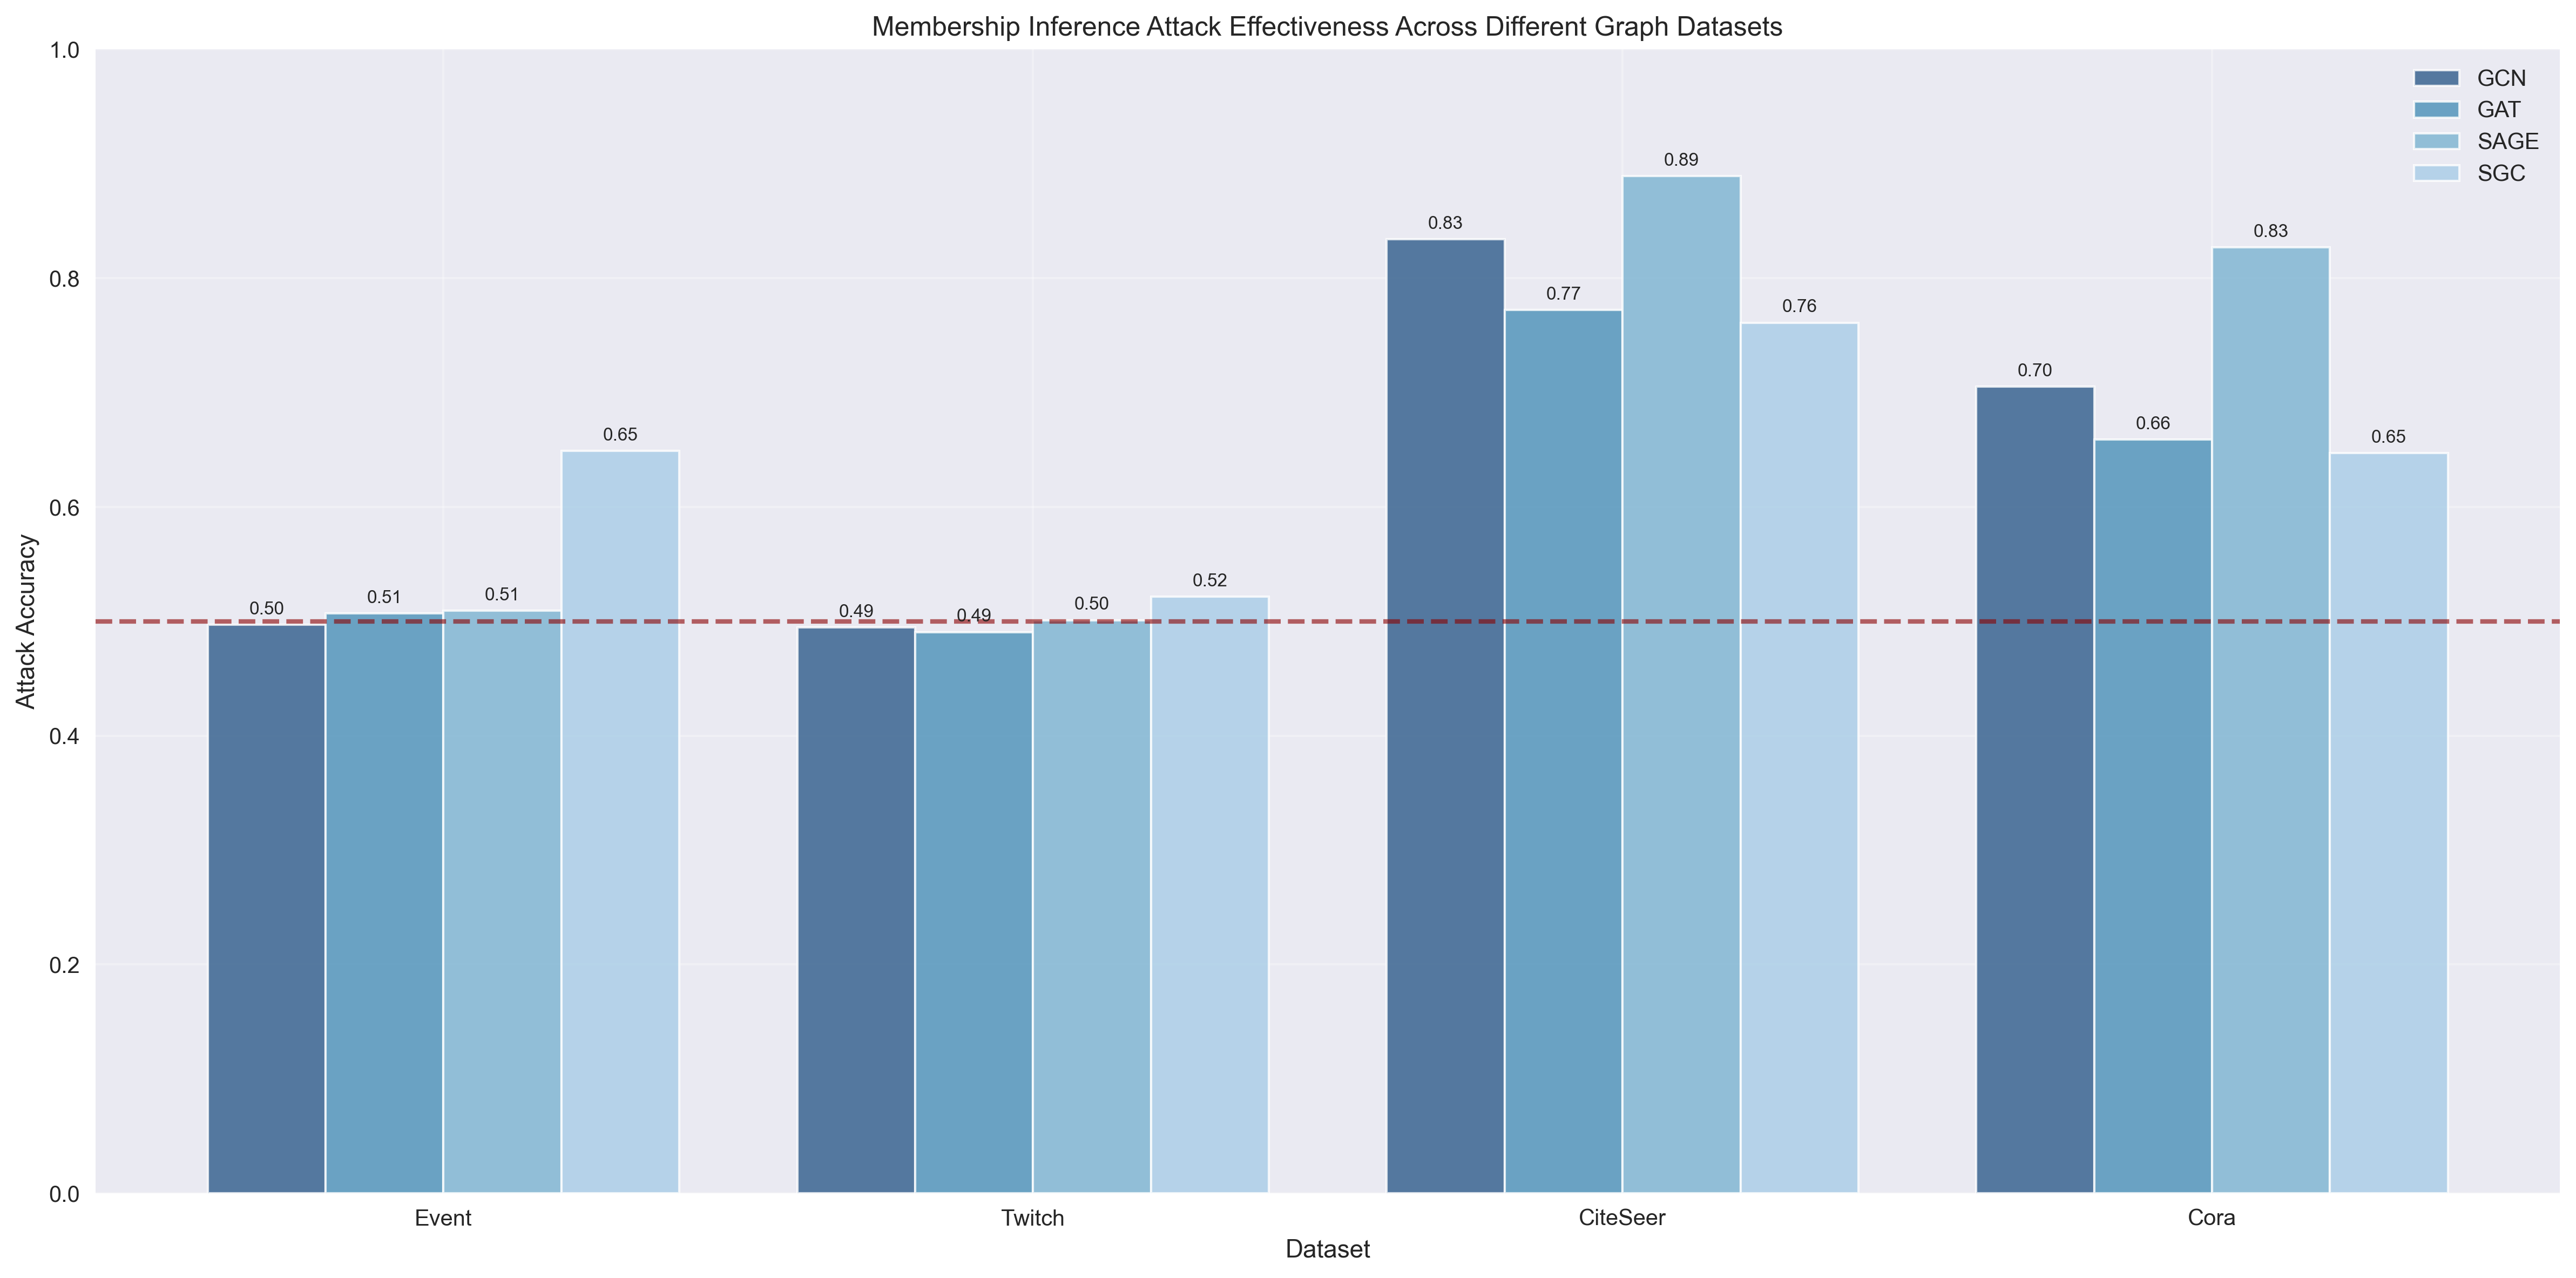
\includegraphics[width=\textwidth]{../Results/visualizations/comprehensive_datasets_comparison.png}
\caption{Attack performance on datasets along with Cora and CiteSeer datasets demonstrates pipeline validity with 70.5-88.9\% accuracy, confirming this implementation correctly identifies membership when both target and shadow models use real data.}
\label{fig:baseline}
\end{figure}

CiteSeer proves more vulnerable (76--89\%) than Cora (65--83\%) across all architectures. GraphSAGE achieves the highest vulnerability on both datasets at 88.9\% on CiteSeer, confirming that this attack methodology exploits overfitting patterns effectively.

\subsection{Architecture Vulnerability Rankings}
Figure \ref{fig:attack-performance} shows clear differences in privacy leakage across GNN architectures on these custom datasets.

\begin{figure}[H]
\centering
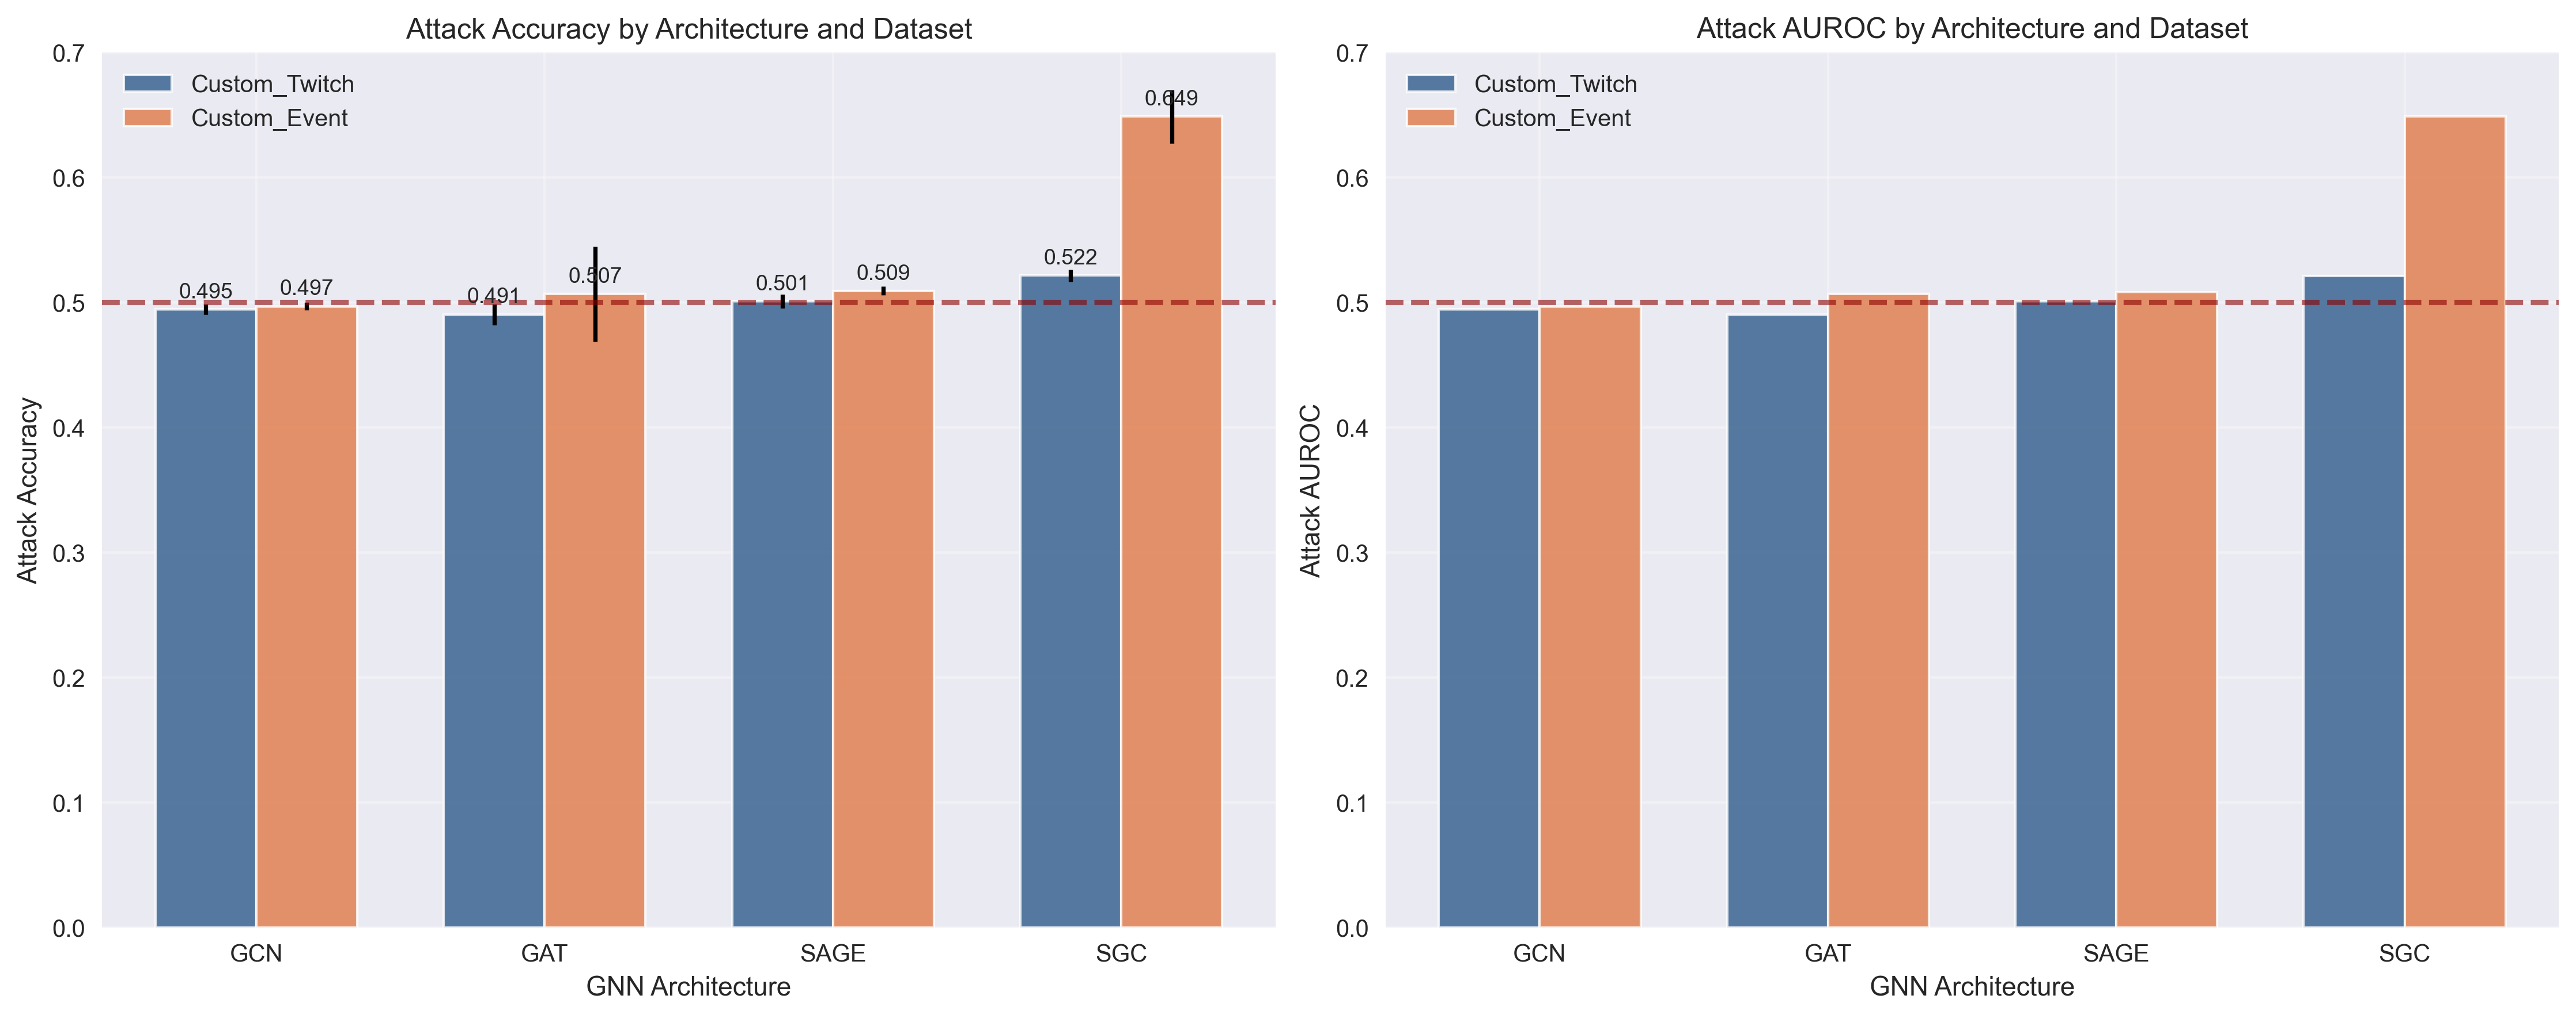
\includegraphics[width=\textwidth]{../Results/visualizations/attack_performance_comparison.png}
\caption{Attack accuracy across GNN architectures for Twitch and Event datasets. The red dashed line marks 50\% (random guessing). AUROC values closely mirror accuracy patterns.}
\label{fig:attack-performance}
\end{figure}

SGC emerges as the most vulnerable architecture, particularly on the Event dataset where it reaches 64.9\% accuracy, well above the 50\% random baseline. SGC's simplified design removes protective layers found in other models, allowing attack models to more easily distinguish training from test data. GCN shows the opposite behavior, maintaining 49.5\% accuracy on both datasets, essentially random performance. This protection comes from GCN's normalization process, which makes it harder to exploit overfitting.

Every model struggles with Twitch data, barely exceeding 52\% accuracy. Yet on Event data, there are dramatic differences, SGC jumps to nearly 65\% while GCN remains at baseline. GAT shows particularly unstable behavior on Event data, with error bars stretching from 45\% to 54\%, suggesting that its attention mechanism sometimes finds exploitable patterns and sometimes doesn't. GraphSAGE sits in the middle with steady 50-51\% accuracy, showing that its neighborhood sampling creates small but consistent privacy leaks.

\subsection{Synthetic Data Effectiveness}
The core contribution of this work, using synthetic graphs for shadow model training, shows measurable but reduced effectiveness compared to traditional approaches. Figure \ref{fig:synthetic-comparison} shows results from an upper bound sanity check experiment where the shadow model was trained on the same data as the target model (real data) to isolate the effect of synthetic vs real shadow training data and establish the maximum possible attack performance.

\begin{figure}[H]
\centering
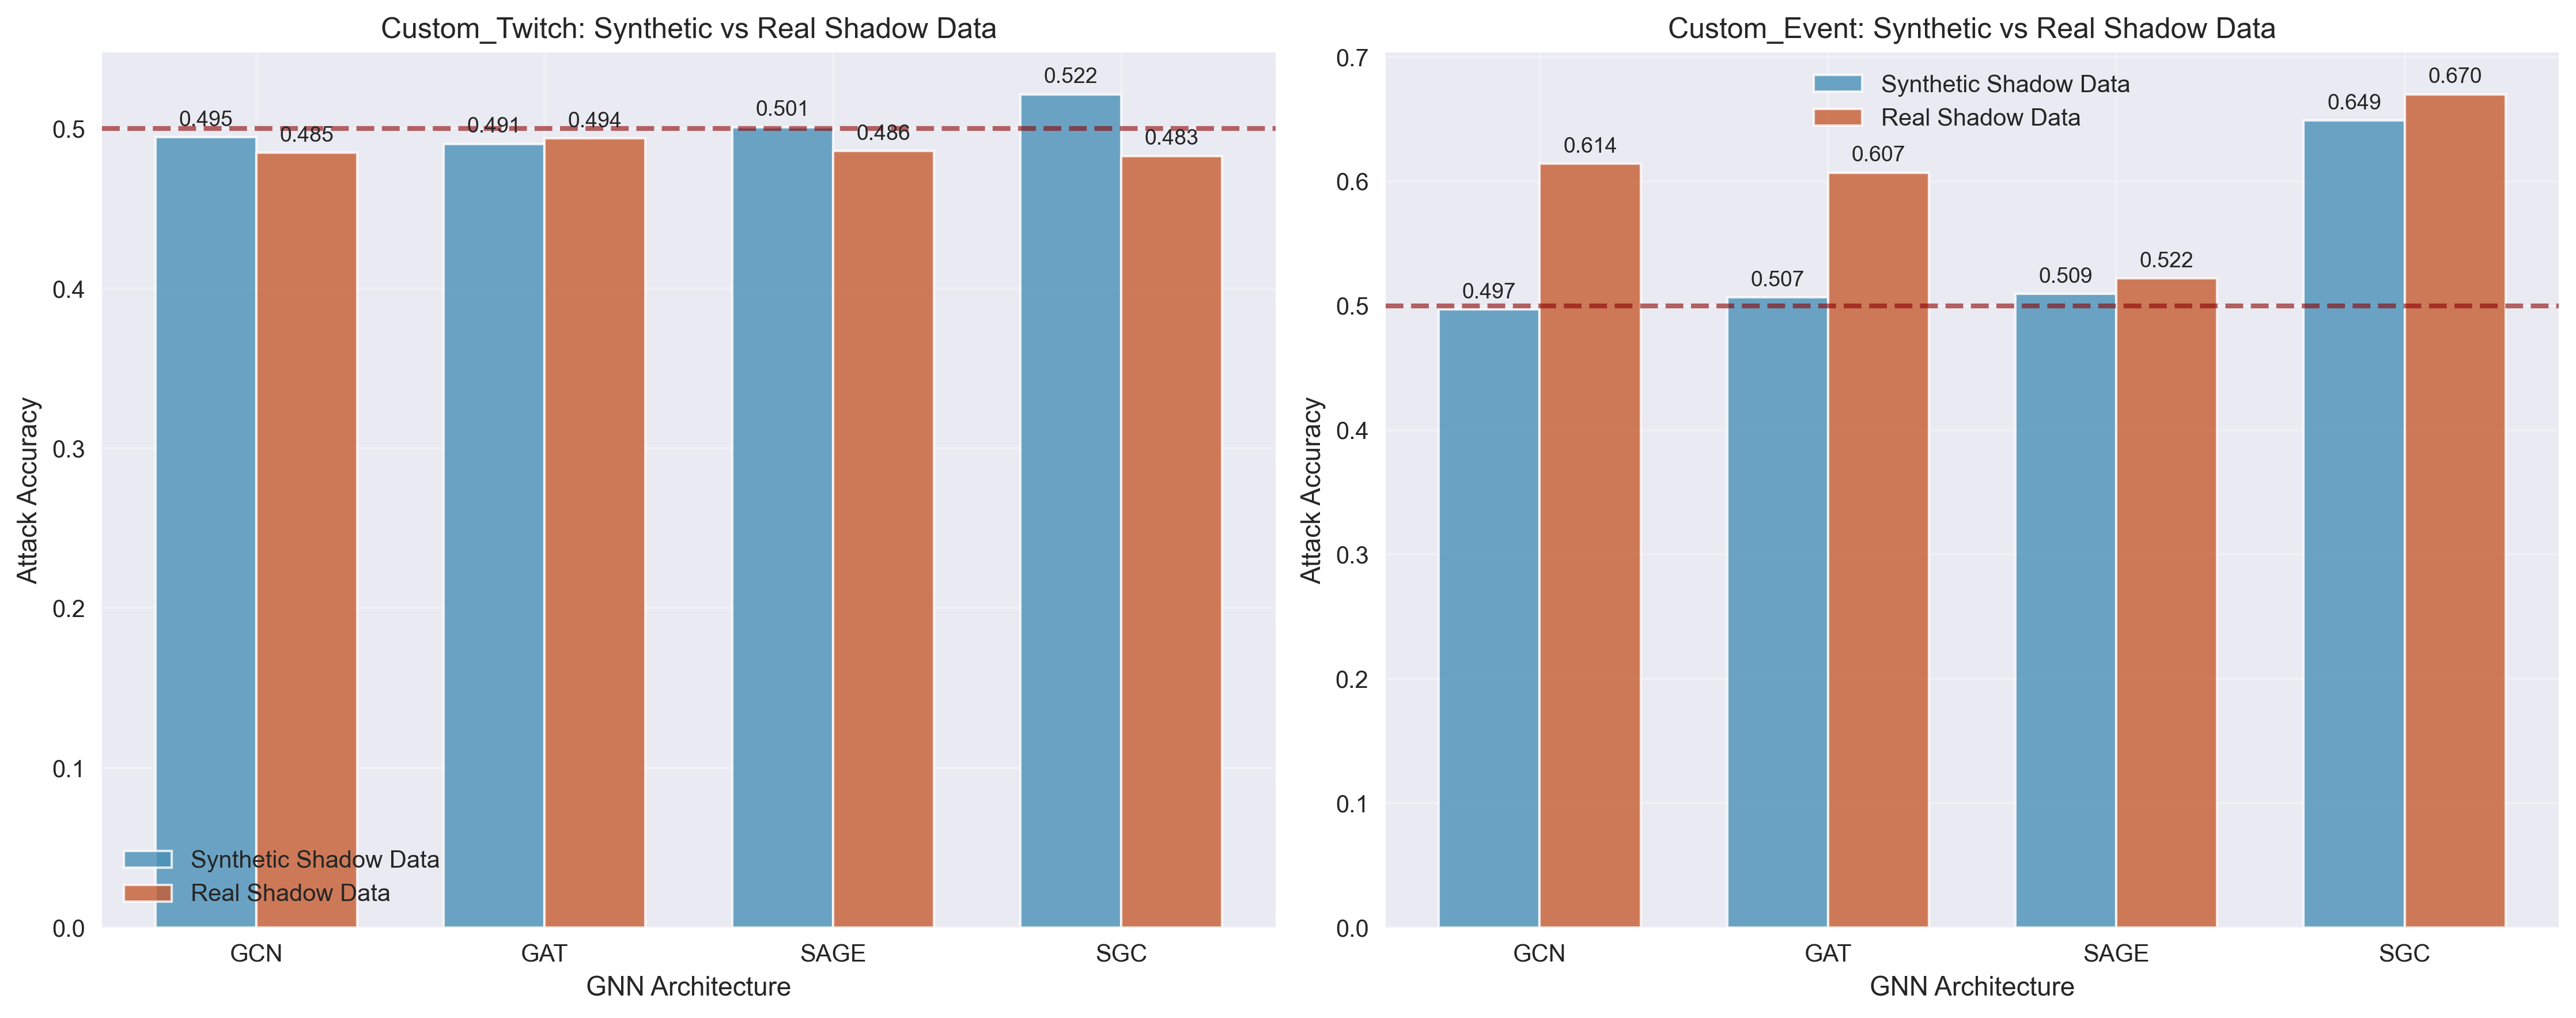
\includegraphics[width=\textwidth]{../Results/visualizations/synthetic_vs_real_comparison.png}
\caption{Synthetic vs real shadow data comparison. Real shadow uses target training data as upper bound sanity check. Event dataset shows consistent degradation (10-15\% drop) when using synthetic data, while Twitch shows minimal difference due to baseline resistance.}
\label{fig:synthetic-comparison}
\end{figure}

Comparing synthetic and real data for shadow model reveals the performance implications of using synthetic data for training. The real shadow data serves as an upper bound sanity check showing maximum achievable attack performance when the shadow model has access to the same data as the target model. On Event data, there is a clear performance drop when switching from this upper bound to synthetic shadow data, SGC drops from 67\% to 65\% accuracy, while GCN falls more dramatically from 61\% to just under 50\%. This 10--15\% degradation indicates that synthetic graphs capture some patterns necessary for successful attacks. However, the results differ with Twitch data, where both approaches perform equally poorly at around 48--52\% accuracy. Twitch's resistance appears unrelated to data quality but reflects something fundamental that prevents models from learning exploitable patterns. Synthetic data maintains roughly 75--80\% of the attack effectiveness on vulnerable datasets, offering a viable alternative when real training data is unavailable.

\subsection{Dataset-Specific Analysis}

\subsubsection{Twitch Dataset}
The Twitch dataset consistently resists membership inference attacks, achieving only ~49\% accuracy across all models and settings, essentially random guessing. Several factors might explain this resistance, though the phenomenon requires further investigation.

Twitch captures streaming behavior rather than static demographics. Unlike the Event dataset where someone's gender or birth year never changes, Twitch features such as view counts and streaming activity fluctuate constantly. This makes it harder for models to memorize specific patterns tied to individual users. Predicting affiliate status might provide too subtle a signal compared to predicting gender from demographic data.

The graph structure also differs significantly between datasets. Twitch follower networks tend to be sparser and more dynamic than social event networks, potentially reducing the neighborhood information that attacks typically exploit. The current approach might not suit data like Twitch. Different attack strategies, feature engineering approaches, or target variables might be more effective. Consistent failure across all architectures suggests this resistance might be fundamental to the data type, though targeted experiments would help determine whether Twitch data is inherently more private or if the methodology needs adaptation.

\subsubsection{Event Dataset}
In contrast to Twitch, the Event dataset proves highly vulnerable to membership inference attacks, with SGC achieving 64.9\% accuracy. This vulnerability stems from the dataset's demographic nature, where features like birth year, gender, and location remain static over time, making it easier for models to memorize specific user patterns. The prediction target, gender classification, creates clear categorical boundaries that attacks can exploit more easily than Twitch's affiliate status. Additionally, social event networks tend to exhibit strong homophily, meaning similar people connect with each other, which amplifies membership signals through the graph structure. The denser connectivity in these networks also provides more neighborhood information that attacks can leverage, creating multiple pathways for privacy leakage that these attacks successfully exploit.

\subsection{Performance Summary Table}

\begin{table}[H]
\centering
\caption{Attack accuracy comparison across experiments (mean ± std over 5 runs). Synthetic shadow is shadow model trained on synthetic data, real shadow uses target training data as upper bound sanity check. Standard datasets (Cora, CiteSeer) validate pipeline correctness.}
\label{tab:performance}
\begin{tabular}{|l|l|c|c|c|}
\hline
\textbf{Experiment} & \textbf{Model} & \textbf{Twitch} & \textbf{Event} & \textbf{Delta} \\
\hline
\multirow{4}{*}{Synthetic Shadow} & GCN & 49.5±0.4\% & 49.7±0.3\% & +0.2\% \\
 & GAT & 49.1±0.8\% & 50.7±3.8\% & +1.6\% \\
 & SAGE & 50.1±0.5\% & 50.9±0.4\% & +0.8\% \\
 & SGC & 52.2±0.4\% & 64.9±1.8\% & +12.7\% \\
\hline
\multirow{4}{*}{Real Shadow} & GCN & 48.5\% & 61.4\% & +12.9\% \\
 & GAT & 49.4\% & 60.7\% & +11.3\% \\
 & SAGE & 48.6\% & 52.2\% & +3.6\% \\
 & SGC & 48.3\% & 67.0\% & +18.7\% \\
\hline
\multirow{4}{*}{Standard Datasets} & GCN & \multicolumn{2}{c|}{Cora: 70.5\%} & CiteSeer: 83.4\% \\
 & GAT & \multicolumn{2}{c|}{Cora: 65.9\%} & CiteSeer: 77.2\% \\
 & SAGE & \multicolumn{2}{c|}{Cora: 82.7\%} & CiteSeer: 88.9\% \\
 & SGC & \multicolumn{2}{c|}{Cora: 64.7\%} & CiteSeer: 76.1\% \\
\hline
\end{tabular}
\end{table}

\section{Evaluation and Analysis}

Comparing these results with the main paper ``Membership Inference Attack on Graph Neural Networks'' by Olatunji et al.\cite{olatunji2021membershipinferenceattackgraph} shows both similarities and key differences in how well attacks work. The original paper showed that GNNs can leak membership information even when they work well on new data, mainly because of structural patterns rather than just overfitting.

The experiments match their finding that GAT is hardest to attack because its attention mechanism changes how the graph looks rather than keeping the actual structure. These results show much lower attack success rates across all models. Where Olatunji et al.\ got 70--88\% attack accuracy on standard datasets like Cora and CiteSeer, this synthetic data approach gets 49--65\% on custom datasets, showing the limitation of using synthetic data instead of real data for training.

The structural information idea from the original work helps explain these dataset differences. Twitch's features change over time and resist the pattern memorization that makes traditional graph datasets easy to attack. Event's fixed demographic features combined with the tendency for similar people to connect create the patterns that the original paper found most vulnerable.

SGC is more vulnerable than GCN, matching the original paper's finding that simpler models keep more patterns that attacks can exploit. This synthetic data setting shows the effect depends on the dataset, strong on vulnerable datasets like Event but weak on resistant ones like Twitch.

\section{Future Work}

The attack models often predict only one class (member or non-member) instead of learning balanced decisions. This is a major problem that needs more research. Future work should focus on building better attack models that make balanced predictions instead of finding false patterns in synthetic training data. This could use better training methods, adversarial training, or combining multiple models that avoid extreme predictions.

Also, it's unclear whether Twitch's resistance comes from behavioral data being naturally more private or from problems with the attack method. Future research should test different attack strategies designed for data that changes over time, including methods that look at sequences and dynamic graph analysis.

\section{Conclusion}
This work introduces a new approach to membership inference attacks on Graph Neural Networks using synthetic graph data for shadow model training, showing that privacy risks exist even when attackers cannot access real training data. Through experiments across four GNN architectures (GCN, GAT, GraphSAGE, SGC) and real world datasets (Twitch, Event), this study achieves attack accuracies of 49--65\% when using synthetic data for training shadow model.

The TSTS (Train on Subgraph, Test on Subgraph) method solves memory problems while enabling practical attacks on large graph datasets. The analysis reveals three key insights: dataset type matters more than model architecture for vulnerability, with behavioral data (Twitch) showing strong resistance while demographic data (Event) remains highly vulnerable. Surprisingly, simpler architectures (SGC) leak more membership information than complex ones (GCN), challenging common beliefs about model complexity and privacy.

Testing on standard benchmarks (Cora, CiteSeer) confirms this method works correctly while showing the unique privacy features of these custom datasets. However, a major problem appears when looking at individual runs: the attack model often predicts almost only one class (member or non-member) instead of learning balanced decisions. For example, some GAT runs get 97\% accuracy on members but only 2.2\% on non-members, while others show the opposite pattern (4\% vs 96\%). This suggests the attack model learns to exploit dataset specific patterns rather than real membership signals.

This bias pattern shows a basic limitation in this attack method. The model may be overfitting to false patterns in the synthetic training data rather than learning strong membership indicators. Twitch's consistent resistance across all attack types suggests that behavioral features that change over time provide natural privacy protection, though this needs more investigation to understand dataset properties versus method limitations.

These findings have important implications for privacy sensitive GNN use. Synthetic data attacks are less effective than traditional approaches but represent a viable threat requiring minimal attacker resources. As graph learning expands into healthcare, finance, and social analytics, both model choice and data type should be considered  in the privacy assessments for the use case.


\bibliography{citations}
\bibliographystyle{unsrt}

\end{document}